\documentclass[12pt, a4paper]{report}
\usepackage{graphicx, array, amsthm, amssymb, amsmath, algorithm, algpseudocode, float, xcolor, thmtools, thmbox, matlab-prettifier, exercise}
\usepackage[english]{babel}

\makeatletter
\renewcommand\thmbox@headstyle[2]{\bfseries #1}
\makeatother
\newtheorem[style=M,bodystyle=\normalfont]{theorem}{Theorem}
\newtheorem[style=M,bodystyle=\normalfont]{corollary}{Corollary}
\newtheorem[style=M,bodystyle=\normalfont]{lemma}{Lemma}
\newtheorem[style=M,bodystyle=\normalfont]{definition}{Definition}

\definecolor{dkgreen}{rgb}{0,0.6,0}
\definecolor{gray}{rgb}{0.5,0.5,0.5}
\definecolor{mauve}{rgb}{0.58,0,0.82}
\lstset{frame=tb,
  language=Java,
  aboveskip=3mm,
  belowskip=3mm,
  showstringspaces=false,
  columns=flexible,
  basicstyle={\small\ttfamily},
  numbers=none,
  numberstyle=\tiny\color{gray},
  keywordstyle=\color{blue},
  commentstyle=\color{dkgreen},
  stringstyle=\color{mauve},
  breaklines=true,
  breakatwhitespace=true,
  tabsize=3
}


\title{Image Analysis And Computer Vision\\ \textit{Exercises}}
\author{Christian Rossi}
\date{Academic Year 2023-2024}

\begin{document}

\maketitle

\newpage

\begin{abstract}
    The topics of the course are: 
    \begin{itemize}
        \item Introduction.
        \item Camera sensors: transduction, optics, geometry, distortion
        \item Basics on Projective geometry: modelling basic primitives (points, lines, planes, conic sections, quadric surfaces) and projective spatial transformations and  projections.
        \item Camera geometry, and single view analysis: calibration, image rectification, localization of 3D models.
        \item Multi-view analysis: 3D shape reconstruction, self-calibration, 3D scene understanding.
        \item Linear filters and convolutions, space-invariant filters, Fourier Transform, sampling and aliasing. 
        \item Nonlinear filters: image morphology and morphology operators (dilate, erode, open, close), median filters.
        \item Edge detection and feature detection techniques. Feature matching and feature tracking along image sequences.
        \item Inferring parametric models from noisy data (including outliers), contour segmentation, clustering, Hough Transform, Ransac (random sample consensus). 
        \item Applications: object tracking, object recognition, classification.
    \end{itemize}
\end{abstract}

\newpage

\tableofcontents

\newpage

\chapter{Introduction to MATLAB}
    \section{Main MATLAB operators}
    To print some string it is possible to use; 
    \begin{lstlisting}[language=Matlab]
% Print the string
disp('string');
% Print the string with C-like syntax
fprintf('string\n%s %d','string',number);
    \end{lstlisting}
    The variables are created as follows: 
    \begin{lstlisting}[language=Matlab]
% Variables are created by assignements
v=3
c='k'
% Data types can be checked
whos v
% Casting to 8-bit integer
v=uint8(v)
    \end{lstlisting}
    The main data types used on MATLAB: double, uint8, and logical. The arrays are defined in the following ways: 
    \begin{lstlisting}[language=Matlab]
% A row vector
r=[1, 2, 3, 4]
% A column vector
c=[1; 2; 3; 4]
% Vectors by regular increment operator
% [start:step:end]
a = [1:2:10];
% A matrix
v=[ 1 2; 
    3 4 ]
    \end{lstlisting}
    It is possible to concatenate arrays: 
    \begin{lstlisting}[language=Matlab]
B=[v', v']
C=[v; v]        
    \end{lstlisting}
    The arrays can be divided in subarrays: 
    \begin{lstlisting}[language=Matlab]
% First row and second column 
v(1,2) 
% The second column of v
v(:,2)
% The first row of v
v(1,:) 
% Some of the columns from 2 to 4
B(:,2:4) 
    \end{lstlisting}
    Some useful mathematical operations are: 
    \begin{lstlisting}[language=Matlab]
% . means elementwise operation
[1 2 3].*[4 5 6]
[1 2 3]+5
[1 2 3]*2 
[1 2 3].*2 
[1 2 3]/2
[1 2 3]./2 
[1 2 3].^2 
% Inner product
[1 2 3]*[4 5 6]' 
% This is the matrix product, returns a matrix
[1 2 3]'*[4 5 6] 
% Functions for rounding functions
ceil(10.56)
floor(10.56)
round(10.56)
% Arithmetic functions
sum([1 2 3 4])
sum([1:4;5:8])
sum([1:4;5:8],2)
    \end{lstlisting}

    \section{Commands for images}
    The images in MATLAB are treated as matrices:
    \begin{lstlisting}[language=Matlab]
im=imread('photo.png');
% Show the image
imshow(im);
% Show two concatenated images orizontally
imshow([im im]);
% Show two concatenated images vertically
imshow([im; im]);
    \end{lstlisting}
    To plot the histogram of the various pixels it is possible to write: 
    \begin{lstlisting}[language=Matlab]
h=hist(im(:),[0: im_length]);
figure(2), stairs([0: im_length], h)
axis tight
    \end{lstlisting}
    It is possible to modify the brightness and contrast with a simple operation:
    \begin{lstlisting}[language=Matlab]
figure(1),imshow(im+50),title('50 graylevels')
figure(1),imshow(im+100),title('100 graylevels')
% contrast modify
eq=double(im-min(im(:)))/double(max(im(:))-min(im(:)))*255;
    \end{lstlisting}
    Image ranges (in the visualization) can be also controlled:
    \begin{lstlisting}[language=Matlab]
imshow(im,[-100 156]);title('more brighness');
imshow(im,[0 156]);title('more brighness and contrast');
imshow(im,[ 100 256]);title('less brighness, more contrast');
imshow(im,[ 100 356]);title('less brighness');
    \end{lstlisting}
    The gamma correction is done in this way: 
    \begin{lstlisting}[language=Matlab]
for gamma= [.04 .1 .2 .4 .7 1 1.5 2.5 5 10 25]
    y=x.^gamma;
    plot(x,y,'DisplayName',sprintf('\\gamma=%.2f',gamma));
    % display the text
    text(x(round(end/2)),y(round(end/2)),sprintf('\\gamma=%.2f',gamma));
end
    \end{lstlisting}
    Color is represented by 3 channels (RGB). We can read each channel:
    \begin{lstlisting}[language=Matlab]
% Red channel
imr=im(:,:,1);
% Green channel
imr=im(:,:,2);
% Blue channel
imr=im(:,:,3);
    \end{lstlisting}

    \newpage

\chapter{Laboratory session I}
\begin{Exercise}[label=1]
    Elaborate the following image called "checkerboard.png": 
    \begin{figure}[H]
        \centering
        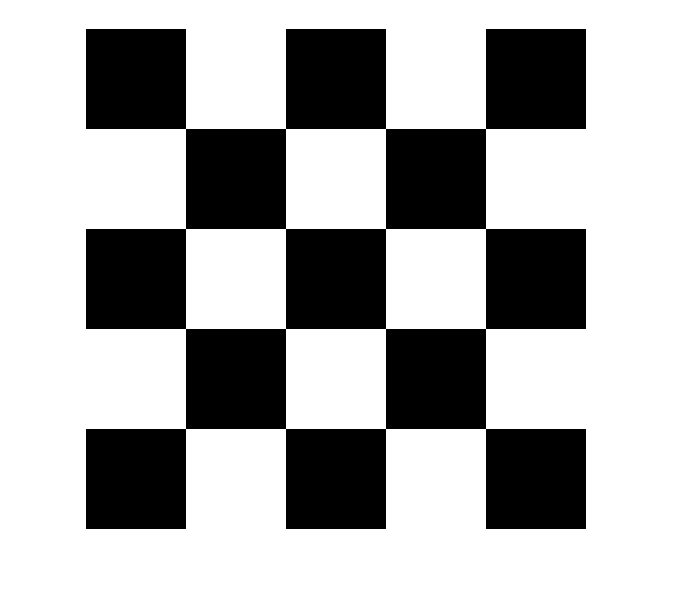
\includegraphics[width=0.5\linewidth]{images/checkerboard.png}
    \end{figure}
\end{Exercise}
\begin{Answer}[ref=1]
    Initially, we have to load the image in a matrix: 
    \begin{lstlisting}[language=Matlab]
I=imread('checkerboard.png');
FNT_SZ=28;
    \end{lstlisting}
    We now want to manually select four points and save them in homogeneous coordinates: 
    \begin{lstlisting}[language=Matlab]
figure(1), imshow(I);
hold on;
[x,y]=getpts();
a=[x(1);y(1);1];
b=[x(2);y(2);1];
c=[x(3);y(3);1];
d=[x(4);y(4);1];
    \end{lstlisting}
    And now we can show the points label on the picture with: 
    \begin{lstlisting}[language=Matlab]
text(a(1),a(2),'a','FontSize',FNT_SZ,'Color','b')
text(b(1),b(2),'b','FontSize',FNT_SZ,'Color','b')
text(c(1),c(2),'c','FontSize',FNT_SZ,'Color','b')
text(d(1),d(2),'d','FontSize',FNT_SZ,'Color','b')
    \end{lstlisting}
    We now define the lines passing through these points: 
    \begin{lstlisting}[language=Matlab]
lab=cross(a,b); 
lad=cross(a,d); 
lac=cross(a,c); 
lcd=cross(c,d);
    \end{lstlisting}
    Intersect these lines with the image borders
    \begin{lstlisting}[language=Matlab]
r1=[0;1;-1];       % Parameters of top-most row
r500=[0;1;-500];   % Parameters of bottom row
c1=[1;0;-1];       % Parameters of left-most column
c500=[1;0;-500];   % Parameters of right-most column
% Intersection between lab and the first column
x1=cross(c1,lab); 
x1=x1/x1(3); 
text(x1(1),x1(2),'x1','FontSize',FNT_SZ,'Color','b')
% Same with the right most column
x500=cross(c500,lab);
x500=x500/x500(3);
text(x500(1),x500(2),'x500','FontSize',FNT_SZ,'Color','b')
plot([x1(1),x500(1)],[x1(2),x500(2)],'LineWidth',3)
        \end{lstlisting}
    Compute the angles on these images:
    \begin{lstlisting}[language=Matlab]
computeEuclideanAngles(lab,lac) 
computeEuclideanAngles(lab,lcd) 
computeEuclideanAngles(lab,lad) 
    \end{lstlisting}
    Verify the proporty any linear combination of $a,b$ belongs to lab: 
    \begin{lstlisting}[language=Matlab]
lambda=rand(1);
mu=1-lambda;
p= lambda*a+mu*b;
p'*lab
p=p/p(3);
text(p(1),p(2),'p','FontSize',FNT_SZ,'Color','b')
    \end{lstlisting}
    Intersect parallel lines
    \begin{lstlisting}[language=Matlab]
vac=cross(lab,lcd)
vac=vac/vac(3) 
vab=cross(r1,r500)
vad=cross(c1,c500)
    \end{lstlisting}

\end{Answer}

    \newpage

    \begin{Exercise}[label=2]
        Elaborate the following image called "simplecube-letters.png": 
        \begin{figure}[H]
            \centering
            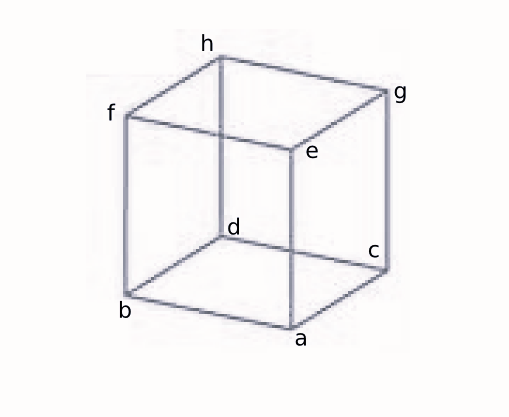
\includegraphics[width=0.5\linewidth]{images/simplecube-letters.png}
        \end{figure}
        And the following image called "buildingSmall.png": 
        \begin{figure}[H]
            \centering
            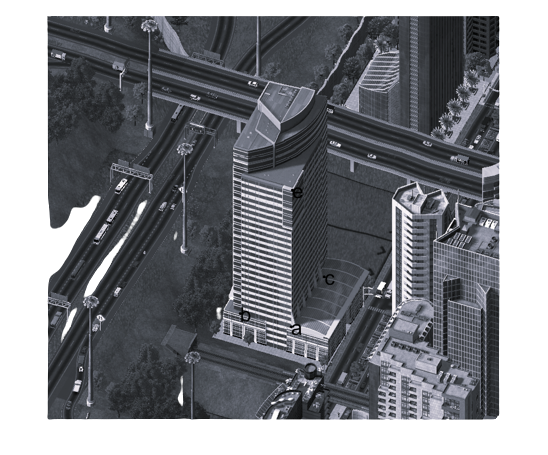
\includegraphics[width=0.5\linewidth]{images/buildingSmall.png}
        \end{figure}
    \end{Exercise}
    \begin{Answer}[ref=2]
        Initially, we have to load the image in a matrix: 
        \begin{lstlisting}[language=Matlab]
figure(1),imshow(imread('simplecube-letters.png'));
        \end{lstlisting}
        Data entering: 
        \begin{lstlisting}[language=Matlab]
figure(2),imshow(imread('buildingSmall.png'))
hold on;
[x y]=getpts
plot(x,y,'.w','MarkerSize',12,'LineWidth',3);
a=[x(1) y(1) 1]';
text(a(1),a(2),'a','FontSize',FNT_SZ,'Color','w')
b=[x(2) y(2) 1]';
text(b(1),b(2),'b','FontSize',FNT_SZ,'Color','w')
c=[x(3) y(3) 1]';
text(c(1),c(2),'c','FontSize',FNT_SZ,'Color','w')
e=[x(4) y(4) 1]';
text(e(1),e(2),'e','FontSize',FNT_SZ,'Color','w')
        \end{lstlisting}
        Finding some lines: 
        \begin{lstlisting}[language=Matlab]
lab=cross(a,b)
lac=cross(a,c)
lae=cross(a,e)
        \end{lstlisting}
        The incidence equation is staisfied if one of the following operations are null: 
        \begin{lstlisting}[language=Matlab]
lab'*a
lab'*b
lac'*a
lac'*c
lae'*a
lae'*e
        \end{lstlisting}  
        We now need to compute the line parallel to ab and passing through c. In order to do this, we create the line at infinity. 
        Then, we find the directions of segments by ab, ac and ae intersecting their lines with the line at infinity. 
        \begin{lstlisting}[language=Matlab]
linf=[0 0 1]';
dab=cross(lab,linf)
dac=cross(lac,linf)
dae=cross(lae,linf)
        \end{lstlisting}
        dab, dac and dae are points at the infinity, which represent directions. All lines with a given direction pass through the corresponding point at the infinity. 
        We can then find the lines containing segments bd and cd.
        \begin{lstlisting}[language=Matlab]
lbd=cross(b,dac);
lcd=cross(c,dab);
        \end{lstlisting}
        point d is now found by just intersecting lbd and lcd
        \begin{lstlisting}[language=Matlab]
d=cross(lbd,lcd);
        \end{lstlisting}
        We normalize d's coordinates so that we can read its cartesian coordinates in d(1) and d(2). We plot the point with a blue circle.
        \begin{lstlisting}[language=Matlab]
d=d/d(3);
plot(d(1),d(2),'.b','MarkerSize',12);
text(d(1),d(2),'d','FontSize',FNT_SZ,'Color','w')
        \end{lstlisting}
        The rest of the procedure is straightforward, and follows exactly the same technique.
        \begin{lstlisting}[language=Matlab]
lbf=cross(b,dae);
lcg=cross(c,dae);
ldh=cross(d,dae);
lef=cross(e,dab);
leg=cross(e,dac);
f=cross(lbf,lef);
g=cross(lcg,leg);
lfh=cross(f,dac);
h=cross(lfh,ldh);
f=f/f(3);
g=g/g(3);
h=h/h(3);
plot(f(1),f(2),'.w','MarkerSize',12,'LineWidth',3); 
text(f(1),f(2),'f','FontSize',FNT_SZ,'Color','w')
plot(g(1),g(2),'.w','MarkerSize',12,'LineWidth',3); 
text(g(1),g(2),'g','FontSize',FNT_SZ,'Color','w')
plot(h(1),h(2),'.w','MarkerSize',12, 'LineWidth',3);
text(h(1),h(2),'h','FontSize',FNT_SZ,'Color','w')
        \end{lstlisting}
        We can now finally draw the cube: 
        \begin{lstlisting}[language=Matlab]
myline=[a';b';d';c';a'];
line(myline(:,1),myline(:,2),'LineWidth',5);
myline=[e';f';h';g';e'];
line(myline(:,1),myline(:,2),'LineWidth',5);
myline=[a';e'];
line(myline(:,1),myline(:,2),'LineWidth',5);
myline=[b';f'];
line(myline(:,1),myline(:,2),'LineWidth',5);
myline=[c';g'];
line(myline(:,1),myline(:,2),'LineWidth',5);
myline=[d';h'];
line(myline(:,1),myline(:,2),'LineWidth',5);
hold off
        \end{lstlisting}
    \end{Answer}
\end{document}